\subsection{Understanding S Parameter Subscripting: A Cheerful Dive!}

\begin{tcolorbox}[colback=gray!10, colframe=black, title=E4B07]
What do the subscripts of S parameters represent?
\begin{enumerate}[label=\Alph*.]
    \item \textbf{The port or ports at which measurements are made}
    \item The relative time between measurements
    \item Relative quality of the data
    \item Frequency order of the measurements
\end{enumerate} \end{tcolorbox}

\subsubsection{Elaboration on Related Concepts}

The S parameters, or scattering parameters, are fundamental in the field of radio frequency (RF) and microwave engineering, particularly when analyzing the behavior of electrical networks. The subscripts used in S parameters typically designate the ports of a network and indicate the directional nature of the measurements taken.

In an N-port network, the S-parameters are defined as follows:
- \( S_{ij} \) denotes the reflection or transmission coefficient from port \( j \) to port \( i \), hence:
  - \( S_{11} \) represents the input reflection coefficient at port 1,
  - \( S_{21} \) represents the forward transmission coefficient from port 1 to port 2, and so forth.

The correct answer, A, highlights that these subscripts identify the specific ports involved in the measurements, which is vital for understanding how signals propagate through and are reflected by the network.

\subsubsection{Concepts Required to Answer the Question}
To fully understand the question and the answer, one would require knowledge of the following concepts:

1. \textbf{Ports in Electrical Networks}: Understanding what a port is—a point at which an electrical or optical signal can enter or exit a device or circuit.
2. \textbf{Transmission and Reflection Coefficients}: Familiarity with how signals behave when they encounter an interface, which leads to partial reflection and criteria for transmission.
3. \textbf{Matrix Representation of S Parameters}: Knowing how S-parameters are organized in matrix form helps in understanding interactions within complex networks.

\subsubsection{Example Calculation}
If we wish to analyze a two-port network's S-parameters through measurements, we could collect the following data:
- The input power at port 1 is set to 1 W.
- The reflected power from port 1 is measured as 0.1 W.
- The transmitted power from port 1 to port 2 is measured as 0.8 W.

Calculating \( S_{11} \) and \( S_{21} \):
\[
S_{11} = \frac{\text{Reflected Power}}{\text{Incident Power}} = \frac{0.1 \, \text{W}}{1 \, \text{W}} = 0.1
\]
\[
S_{21} = \frac{\text{Transmitted Power}}{\text{Incident Power}} = \frac{0.8 \, \text{W}}{1 \, \text{W}} = 0.8
\]

A visual representation of this two-port S-parameter network might help clarify the concepts further. Here's a simple diagram illustrating the ports and signal flow using TikZ:

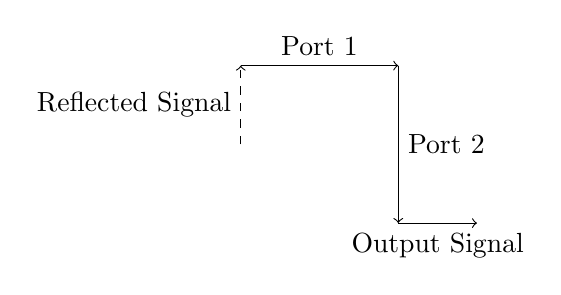
\begin{tikzpicture}
    \draw[->] (0,0) -- (2,0) node[midway, above] {Port 1};
    \draw[->] (2,0) -- (2,-2) node[midway, right] {Port 2};
    \draw[->, dashed] (0,-1) -- (0,0) node[midway, left] {Reflected Signal};
    \draw[->] (2,-2) -- (3,-2) node[midway, below] {Output Signal};
\end{tikzpicture}
